\documentclass[../main.tex]{subfiles}

\begin{document}
%--Copyright oldal----------------------------------------
\thispagestyle{empty}
Szerzői jog \textcopyright ~Tar Dániel, 2018.
\newpage

% --Feladatkiírás lapja------------------------------------
\thispagestyle{empty}
\includepdf[pages=-, offset=80 -75]{resources/tard_feladatkiiras}
% \begin{center}
%     Ide kell befűzni az eredeti feladatkiírási lapot!
% \end{center}
\newpage

%--Nyilatkozatok------------------------------------------
% 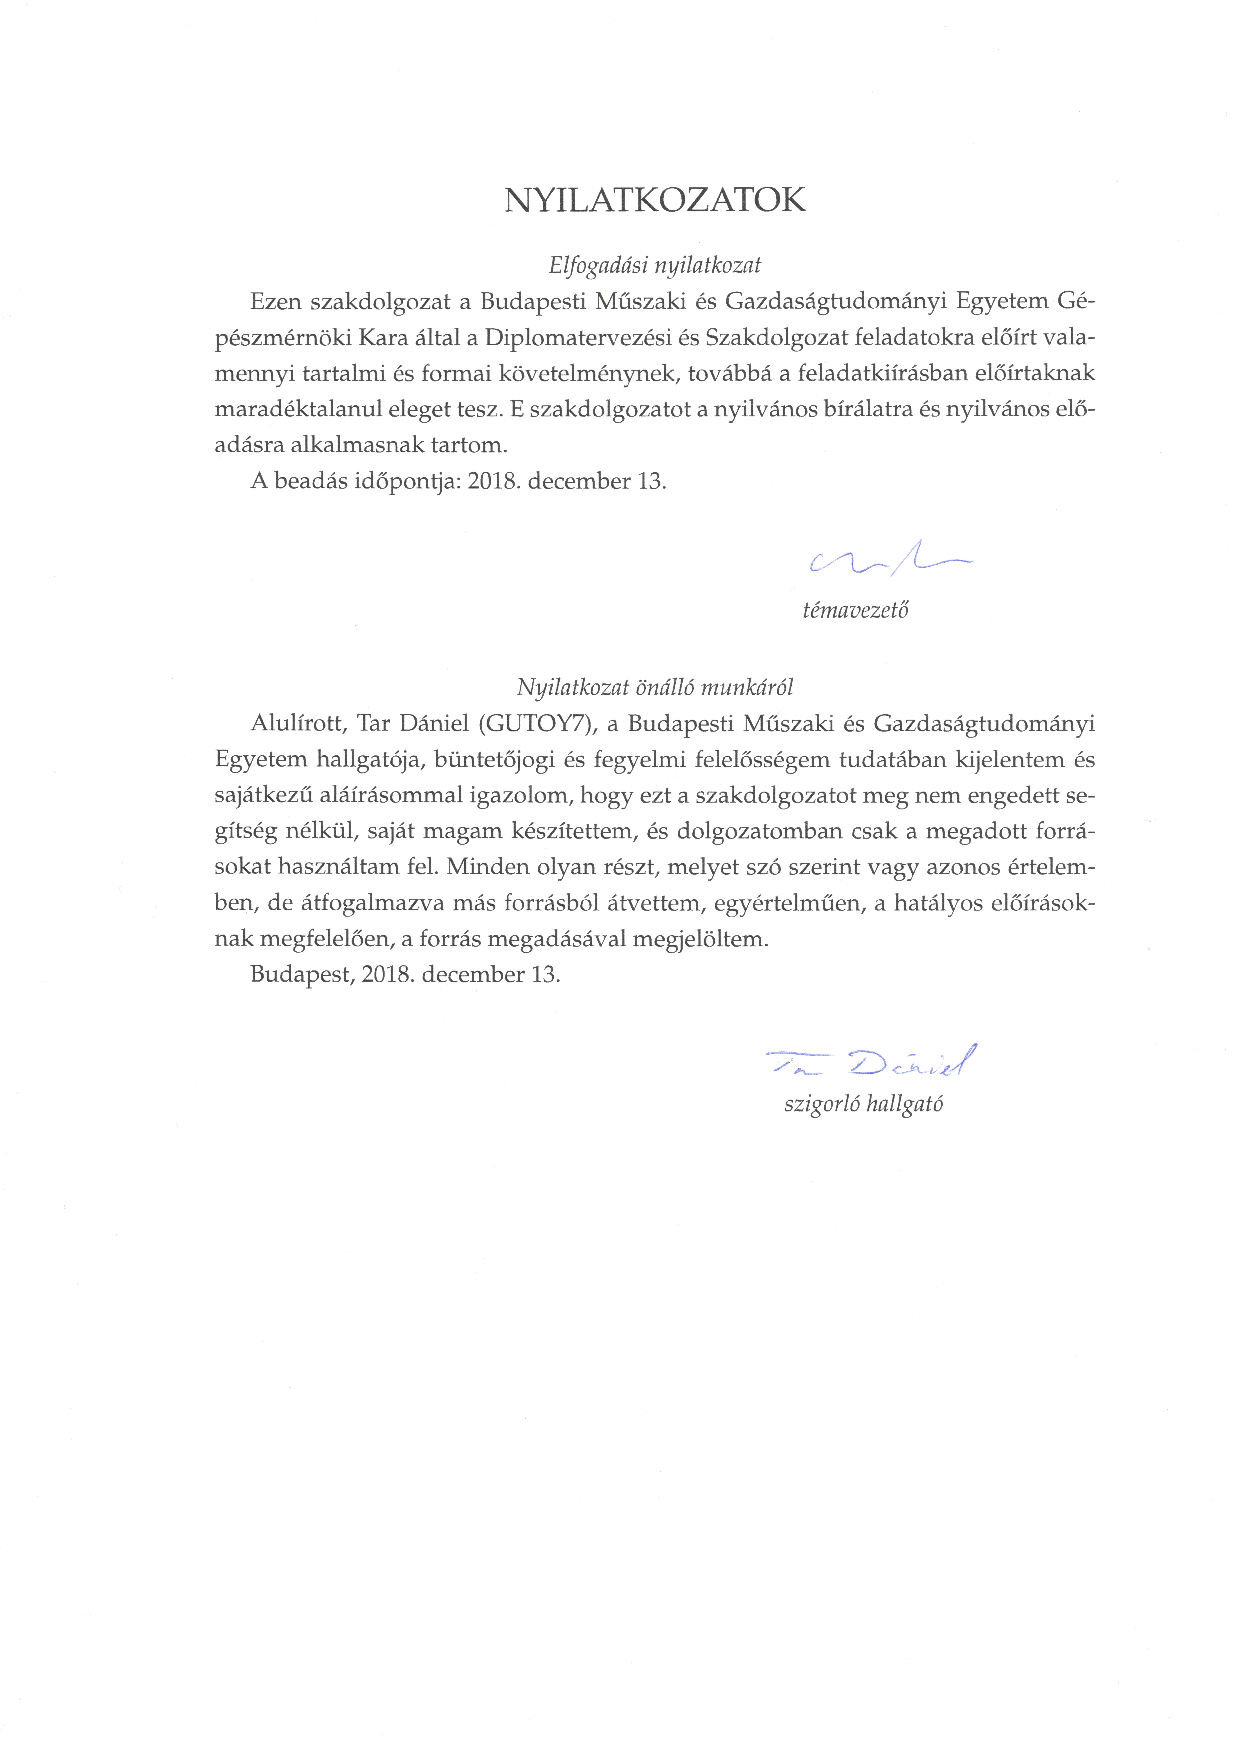
\includepdf[pages=-, offset=80 -75]{resources/tard_nyilatkozatok}
\thispagestyle{plain}
\begin{center}
    \Large \MakeUppercase{Nyilatkozatok}
\end{center}

% {\centering \itshape Beadhatósági nyilatkozat \par}
% A jelen szakdolgozat az üzem által elvárt szakmai színvonalnak mind tartalmilag, mind formailag megfelel, beadható.

% Kelt, Budapest, \today

% {\hspace{0.4\textwidth} Az üzem részéről:}\\[1cm]

% {\hspace{0.6\textwidth} \itshape üzemi konzulens}\\[0.1cm]

{\centering \itshape Elfogadási nyilatkozat \par}
Ezen szakdolgozat a Budapesti Műszaki és Gazdaságtudományi Egyetem Gépészmérnöki Kara által a Diplomatervezési és Szakdolgozat feladatokra előírt valamennyi tartalmi és formai követelménynek, továbbá a feladatkiírásban előírtaknak maradéktalanul eleget tesz. E szakdolgozatot a nyilvános bírálatra és nyilvános előadásra alkalmasnak tartom. 

A beadás időpontja: \today\\[1cm]

{\hspace{0.62\textwidth} \itshape témavezető}\\[0.1cm]

{\centering \itshape Nyilatkozat önálló munkáról \par}
Alulírott, \textit{\myname} (\myneptun), a Budapesti Műszaki és Gazdaságtudományi Egyetem hallgatója, büntetőjogi és fegyelmi felelősségem tudatában kijelentem és sajátkezű aláírásommal igazolom, hogy ezt a szakdolgozatot meg nem engedett segítség nélkül, saját magam készítettem, és dolgozatomban csak a megadott forrásokat használtam fel. Minden olyan részt, melyet szó szerint vagy azonos értelemben, de átfogalmazva más forrásból átvettem, egyértelműen, a hatályos előírásoknak megfelelően, a forrás megadásával megjelöltem.

{Budapest, \today}\\[1cm]

{\hspace{0.6\textwidth} \itshape szigorló hallgató}
%--End of Nyilatkozatok------------------------------------------


\end{document}